% !TEX encoding = UTF-8 Unicode
\chapter{Eine Modellformulierung für Auftragsannahme- und Lagerhaltungsentscheidungen bei auftragsbezogenen Instandhaltungsprozessen}\label{HauptteilDP}
\markboth{5 Modellformulierung}{}
\setcounter{footnote}{86}

\section{Modellannahmen zur Berücksichtigung von Lagerhaltungsentscheidungen}

%\subsection{Beachtung von Produktanfragen für nachfolgende Buchungsabschnitte}

% Lagerhaltungsparameter y
Zur Berücksichtigung von Lagerhaltungsentscheidungen im Netzwerk RM wird für die Erweiterung der Gleichung \eqref{DP} der Parameter für den Lagerbestands $y_{h}$ benötigt. In Bezug auf das Ausgangsproblem der Lagerhaltungsentscheidung ist dieser Schritt der Modellerweiterung nötig, damit ein Parameter für bereits reparierte Produkte im Modell vorhanden ist. Das Modell berücksichtigt Produkte die im gleichen Verhältnis zu einer jeweiligen Ressource $h\in\mathcal{H}$ substituierbar sind. Es existiert damit für jede Ressource $h\in\mathcal{H}$ ein möglicher Lagerbestand $y_h$. Die Obergrenze eines jeden Lagerbestands wird als Parameter $y_{h}^{max}$ beschrieben. Die einzelnen Lagerbestände können als Vektor $\textbf{y}$ bzw. $\textbf{y}^{max}$ zusammengefasst werden. %In der Modellerweiterung wird davon ausgegangen, dass Kapazitäten $c_{h}$ einer Ressource $h$ verwendet werden können, damit der Lagerbestand an Ressourcen $y_{h}$ erhöht wird. Es handelt sich damit um eine Art der Vorarbeit der Leistung. Die einzelnen Bestandteile des Produkts werden auf Lager gelegt, damit diese zu einem späteren Zeitpunkt Verwendung finden. In dieser Modellerweiterung wird davon ausgegangen, dass ein komplettes Bündel des Produkts $j$ auf Lager gelegt wird.


% Grundaufbau des Modells
Das Modell für Auftragsannahme- und Lagerhaltungsentscheidungen soll es ermöglichen ertragsarme Anfragen $j$ nach auftragsbezogenen Instandhaltungsprozessen abzulehnen und eine Erhöhung des Lagerbestands $y_{h}$ über den Parameter $a_{hj}$ zu ermöglichen, sofern die Annahme dieser Anfragen relevante Ressourcenkapazitäten $c_{h}$ für im Buchungshorizonts $T$ spätere eintreffende ertragreiche Anfragen $j$ reduzieren würde. Weiter ist eine Annahme von Anfragen $j$ nach Instandhaltungsprozessen über den Lagerparameter $y_{h}$ möglich, indem anstelle der Kapazitäts- eine Lagerreduktion erfolgt. Der Parameter $y_{h}$ wird bei der Annahme via Lagerbestand um den Parameter $a_{hj}$ reduziert. Damit fungiert in diesem Modell der Parameter $a_{hj}$ als Bestandsveränderung der Kapazitäten oder der Lagerbestände. 

% Leistungsperioden
Für die Modellerweiterung werden Produktanfragen betrachtet, die für bestimmte Leistungserstellungszeitpunkte vorgesehen sind. Ein Leistungserstellungszeitpunkt wird durch den Parameter $\hat{t}$ definiert. Damit existiert für eine jede Ressource $h\in\mathcal{H}$ eine Kapazität $c_h^{\hat t}$ und ein Lagerbestand $y_h^{\hat t}$ für einen jeden Leistungserstellungszeitpunkt $\hat{t}$. Damit wird den Parametern für den Kapazitäts- und Lagerbestand der hochgestellte Index zum zugehörigen Buchungsabschnitt $\hat{t}$ ergänzt. Die Menge aller Leistungserstellungszeitpunkte wird mit dem Parameter $\hat T$ abgebildet. Zur Vereinfachung des Modells wird nur eine einzelne Ressource $h$ über den gesamten Buchungshorizont betrachtet. Der jeweilige Eintrag im Vektor $\textbf{c}^{\hat t}$ entspricht somit der Kapazität $c_h^{\hat t}$ der Ressource $h=1$ zum Leisungserstellungszeitpunkt $\hat{t}$. Der aktuell betrachtete Leistungserstellungszeitpunkt $\hat t$ wird ermittelt durch nachfolgende Gleichung:\footnote{Vgl. \cite{lars}.}

\begin{equation}\label{lp}
\hat t = \floor*{\frac{\max(T) -t}{\frac{\max(T)}{\max\hat{(T)}}}}+1
\end{equation}

Es gilt die Annahme, dass die Leistungserstellungszeitpunkte $\hat t\in \hat T$ gleichmäßig über den gesamten Buchungshorizont $T$ aufgeteilt sind. Die bis zur Leistungserstellung benötigten Perioden werden durch Division des Buchungshorizonts $T$ und der Leistungszeitpunkte $\hat T$ ermittelt. Dabei gilt die Bedingung, dass der Buchungshorizont $T$ durch die Anzahl der Leistungszeitpunkte $\hat t$ ganzzahlig teilbar sein muss.

% Kapazitätsverbrauch
Der Kapazitätsverbrauch $a_{hj}^{\hat t}$ einer Produktanfrage $j$ beschreibt mit dem jeweiligen Eintrag den Zeitpunkt der Erfüllung der Anfrage und dem daraus resultierenden Verbrauch der Ressource $h=1$ zur Leistungserstellung $\hat t$. Sei $\tilde{j}$ eine Anfrage nach einem Produkt für diese Modellerweiterung, dann beschreibt der Parameter $\textbf{a}_{\tilde{j}}^{\hat t}=(0,1,0)$, dass die Erfüllung der Anfrage für den Leistungserstellungszeitpunkt $\hat{t}=2$ vorgesehen ist.  Bspw. erfolgt für eine Anfrage $\tilde j$ mit einem Kapazitätsverbrauch $\textbf{a}^{\hat t}_{\tilde{j}}=(0,1,0)$ für einen Buchungshorizont in Länge von $T=15$ eine Leistungserstellung der Anfrage $j$ mit Ablauf der sechsten Periode $t$. Damit wird ab der Periode $t=5$ eine neue Leistungserstellung betrachtet.\\[.5cm]

% Vorzeitiges Buchen
Dem modifizierten Modell soll es erlaubt sein, durch Betrachten der Leistungserstellungszeitpunkte $\hat t \in \hat T$ die vorzeitige Inanspruchnahme von Kapazitäten $c_{h}^{\hat t}$ für Produktanfragen $j$ für nachfolgende Leistungserstellungszeitpunkte $\hat{t}$ zu ermöglichen, was der Annahme des Instandhaltungsauftrags entspricht. Diese Veränderung resultiert aus der Tatsache, dass die Bestandsveränderung $\textbf{a}_j^{\hat t}$ einer Anfrage $j$ bereits vor dem eigentlichen Leistungserstellungszeitpunkt $\hat t$ den Zugriff auf die Kapazität $\textbf{c}^{\hat t}$ oder den Lagerbestand $\textbf{y}^{\hat t}$ erlaubt. Jedoch darf kein Zugriff des Parameters $\textbf{a}_j^{\hat t}$ nach Überschreitung des Leistungserstellungszeitpunkts $\hat t$ auf die jeweiligen Bestände $\textbf{c}^{\hat t}$ bzw. $\textbf{y}^{\hat t}$ erfolgen. Anders formuliert bedeutet dies, dass nicht beanspruchte Kapazitäten $c_{h}^{\hat t}$ für vergangene Leistungserstellungszeitpunkte $\hat t$ nicht mehr für weitere Auftragsannahme verwendet werden dürfen. Diese Eigenschaft wird mit der Wahrscheinlichkeit $p_j(t)$ für die jeweiligen Anfragen $j\in\mathcal{J}$ gesteuert. Dabei ist der Zeitpunkt an dem die erste Produktanfrage $j$ eintrifft unerheblich. Mit dieser Modellerweiterung ist eine umfassendere Betrachtung der Auftragsannahme in der Auftragsfertigung als im Vergleich zum Grundmodell \ref{DP} aus Kapitel \ref{KapitelDP} möglich.\footnote{Vgl. \cite{lars}.} Abbildung \ref{LP2} zeigt die Rahmenbedingungen der Modellerweiterung als grafische Darstellung. Dabei soll der Zusammenhang von Buchungsperioden und der Leistungserstellungszeitpunkte verdeutlicht werden. Ebenfalls zeigt die Abbildung beispielhaft welche Produktanfragen in welchen Zeiträumen eintreffen könnten.

\begin{figure}[h!]
  \begin{center}
    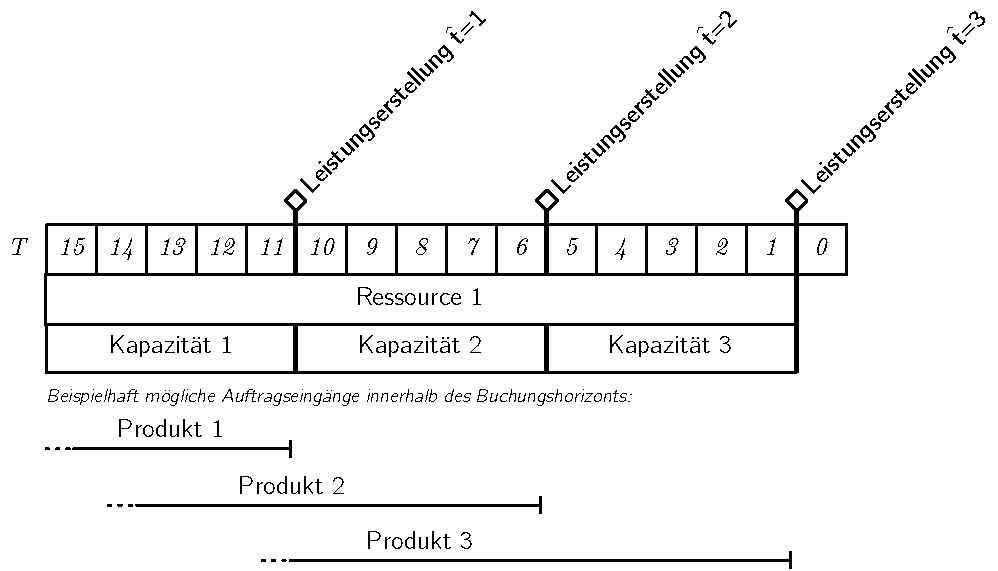
\includegraphics[width=130mm]{Bilder/Leistungsperioden2.pdf}
    \caption{Zusammenhand von Buchungsperioden und den Leistungserstellungszeitpunkten}  \label{LP2}
    {\footnotesize \textbf{In Anlehnung an:} \cite{lars}}. 
  \end{center}
\end{figure}



\section{Mathematische Formulierung eines Modells zur Entscheidungsunterstützung bei Auftragsannahme- und Lagerhaltungsentscheidungen}\label{Umformung}

% Neuer Terme
Für die Modellerweiterung erfolgt die Anpassung der \textit{Bellman'schen Funktionsgleichung}  \eqref{DP} um die Entscheidung der Lagerentnahme in Form des Terms $r_{j} + V(\textbf{c}^{\hat t}, \textbf{y}^{\hat t}-Y(\textbf{a}_j^{\hat t}, \hat t), t-1)$. Der Term beschreibt die Annahme mittels des Lagerbestands. Damit ist es dem Unternehmen möglich entweder die Kapazität oder den Lagerbestand zur Annahme einer Anfrage eines Instandhaltungsprozess in Anspruch zu nehmen. Die Entscheidung der gewollten Ablehnung einer Anfrage $j$ zur Produktion eines Lagerbestand $y_h^{\hat t}$ wird mit dem Term $V(\textbf{c}^{\hat t}-\textbf{a}^{\hat t}_j, \textbf{y}^{\hat t}+Y(\textbf{a}^{\hat t}_j, \hat t +1), t-1)$ dargestellt. Für das Modellformulierung gilt weiterhin, dass eine Ressource und eine Einheit des Lagerbestands im gleichen Verhältnis substituierbar sind.
%Eine Lagerproduktion in der Instandhaltung kann z. B. die vorherige Aufarbeitung von Ressourcen sein, damit für spätere Instandhaltungsaufträge anstelle der Instandsetzung ein Austausch des zu reparierenden Produkts erfolgt.

Sofern eine Reduzierung des Lagerbestand $\textbf{y}^{\hat t}$ als Entscheidung gewählt ist, wird der Lagerparameter bzw. die einzelnen Eintragungen des Vektors des Lagerparameters für alle betreffenden Leistungserstellungszeitpunkte $\hat t\in \hat T$ reduziert. Weiter ist dem Modell gestattet, eine Entscheidung über die Ablehnung einer Anfrage $j$ zu berücksichtigen, bei der aufgrund einer Reduktion der Ressourcenkapazität $\textbf{c}^{\hat t}$ eine Erhöhung des Lagerbestand $\textbf{y}^{\hat t}$ um jeweils des Parameters $\textbf{a}_j^{\hat t}$ möglich ist. Eine Erhöhung des Lagerbestands $\textbf{y}^{\hat t}$ einer jeden Ressource $h$ erfolgt über den gesamten Buchungshorizont und ist ab dem nachfolgenden Leistungserstellungszeitpunkt $\hat t$ verfügbar. %Sei der aktuelle Lagerbestands $\textbf{y}^{\hat t}=(0,0,0)$ über alle Leistungserstellungszeitpunkte $\hat t$. Dann erfolgt durch die Annahme einer Anfrage $j$ mit der Bestandsveränderung $\textbf{a}_j^{\hat t}=(0,1,0)$ eine Erhöhung des Lagerbestand auf $\textbf{y}^{\hat t}=(0,1,1)$, da die Leistung erst nach Erstellung in $\hat{t}=1$ verfügbar ist.

Zur Ermittlung der Veränderung des Lagerbestands aufgrund der Lagerentnahme oder der Lagerproduktion ist die Hilfsfunktion $Y(\textbf{a}_j^{\hat t}, \hat t)$ erforderlich, die den Parameter für den Kapazitätsverbrauch $\textbf{a}_j^{\hat t}$ über alle nachfolgenden Leistungserstellungszeitpunkten kumuliert.\footnote{Vgl. \cite{lars}.} Als Beispiel wird der Kapazitätsverbrauch $\textbf{a}_j^{\hat t}=(0,1,1,0)$ betrachtet. Ein Auftrag $j$ mit einem Verbrauch des vorher aufgeführten Parameters $\textbf{a}_j^{\hat t}$ zeigt eine Leistungserstellung über mehrere Perioden auf. Die Hilfsfunktion zur Ermittlung der Lagerbestandsveränderung berechnet damit eine Veränderung in Höhe des Vektors $Y(\textbf{a}_j^{\hat t}, \hat t)=(0,1,2,2)$. Sofern es sich um eine Veränderung in Form einer Lagerproduktion handelt, ist der Lagerbestand erst zur nachfolgenden Leistungserstellungsperiode $\hat t+ 1$ verfügbar. D. h. die Hilfsfunktion erstellt dem Vektor $Y(\textbf{a}_j^{\hat t}, \hat t +1 )=(0,0,1,2)$. Es muss beachtet werden, dass ein Auftrag $j$ mit einem Kapazitätsverbrauch von $\textbf{a}_j=(0,0,1,2)$ eine Lagererhöhung $Y(\textbf{a}_j, \hat t +1)=(0,0,0,1)$ verursacht. Diese Erhöhung liegt außerhalb des Betrachtungszeitraums. Damit kann zwar ein Teil der Bestandsveränderung für den aktuellen Betrachtungszeitraum genutzt werden, aber der andere Teil geht in dieser Modellformulierung verloren. Eine zusätzliche Betrachtung einer Beanspruchung von Beständen außerhalb des Betrachtungszeitraums (Perioden $t\le0$) in Form von z. B. Lagerentnahmen findet in dieser Arbeit keine Anwendung.

Die mathematische Formulierung der \textit{Bellman'schen Funktionsgleichung} für Auf\-trags\-annahme- und Lagerhaltungsentscheidungen bei auftragsbezogenen Instandhaltungsprozessen wird damit wie folgt beschrieben:
\begin{equation}\label{time}
\begin{alignat*}{2}
V(\textbf{c}^{\hat{t}}, \textbf{y}^{\hat{t}}, t) =\;& \sum_{j \in \mathcal{J}}p_{j}(t)\max[\underbrace{V(\textbf{c}^{\hat{t}}, \textbf{y}^{\hat{t}}, t-1)}_{\text{Ablehnung}}, \underbrace{r_{j} + V(\textbf{c}^{\hat{t}}-\textbf{a}^{\hat t}_j, \textbf{y}^{\hat{t}}, t-1)}_{\text{Annahme via Kapazität}},\\
& \underbrace{r_{j} + V(\textbf{c}^{\hat{t}}, \textbf{y}^{\hat{t}}-Y(\textbf{a}_j^{\hat t},\hat t), t-1)}_{\text{Annahme via Lagerentnahme}}, \underbrace{V(\textbf{c}^{\hat{t}}-\textbf{a}_j^{\hat t}, \textbf{y}^{\hat{t}}+Y(\textbf{a}_j^{\hat t}, \hat t +1), t-1)}_{\text{Ablehnung und Lagerproduktion}}]\\
& + p_{0}(t)\max_{j\in \mathcal{J},\atop p_j(t)>0}[ \underbrace{V(\textbf{c}^{\hat{t}}, \textbf{y}^{\hat{t}}, t-1)}_{\text{Keine Lagerproduktion}},  \underbrace{V(\textbf{c}^{\hat{t}}-\textbf{a}^{\hat t}_j, \textbf{y}^{\hat{t}}+Y(\textbf{a}_j^{\hat t},\hat t +1 ), t-1)}_{\text{Lagerproduktion}}]
\end{alignat*}
\end{equation}

Die Gleichung \eqref{time} zeigt im ersten Term, welche Entscheidungen bzgl. der optimalen Politik möglich sind, sofern eine Anfrage $j\in\mathcal J$ in Abhängigkeit der Wahrscheinlichkeitsverteilung $p_j(t)$ eintrifft. Es wird das Maximum über die Entscheidungen \glqq Ablehnung des Auftrags{\grqq}, \glqq Annahme via Kapazität{\grqq}, \glqq Annahme via Lagerentnahme{\grqq} sowie \glqq Lagerproduktion{\grqq} gewählt. Damit geht aus der Gleichung \eqref{time} hervor, dass es zu jedem Erwartungswert, somit für jedes Teilproblem des Netzwerks, für eine jede Anfrage $j$ die vier Optionen bzw. Entscheidungen existieren. Es gibt damit für eine jede Produktanfrage $j$ im gesamten Netzwerk einen Wert, der die optimale Politik beim Eintreffen einer Anfrage beschreibt. Dieser Wert der optimalen Politik beschreibt die Variable $d_j({\textbf{c}^{\hat t},\textbf{y}^{\hat t},t})\forall j\in\mathcal{J}$. Dieser Variable existiert für jedes Produkt und ist abhängig vom Systemzustand. Ein Systemzustand wird durch die verbleibende Kapazität $\textbf{c}^{\hat t}$ und des Lagerbestands $\textbf{y}^{\hat t}$ zur Periode $t$ beschrieben. Die Variable kann ebenfalls als Vektor $\textbf{d}({\textbf{c}^{\hat t},\textbf{y}^{\hat t},t})$ interpretiert werden und zeigt damit für ein Teilproblem des Netzwerks die optimale Politik über alle möglichen Anfragen. Inhalt des Vektors ist der jeweilige Index der optimalen Politik. Die Variable nimmt den Wert $d_j({\textbf{c}^{\hat t},\textbf{y}^{\hat t},t})=1$ an, sofern die Option der Auftragsannahme via Kapazität den höchsten Erwartungswert liefert und den Wert $d_j({\textbf{c}^{\hat t},\textbf{y}^{\hat t},t})=2$, wenn die Auftragsannahme via Lagerbestand der optimalen Politik entspricht. Sofern die Ablehnung des Auftrags erfolgen soll, aber inkl. der Entscheidung der Lagerproduktion, dann nimmt die Variable $d_j({\textbf{c}^{\hat t},\textbf{y}^{\hat t},t})$ den Wert $3$ an. Sofern die optimale Politik die generelle Ablehnung der Anfrage ist, nimmt die Variable den Wert $d_j({\textbf{c}^{\hat t},\textbf{y}^{\hat t},t})=0$ an.

% Alte und neue Grenzbedingungen
Für die verschiedenen Entscheidungsalternativen existieren unterschiedliche $OC_{j}$, wie aus der Gleichung \eqref{time} zu erkennen ist. Damit trägt der Parameter $OC_{j}$ den Superskript $d$ für die jeweilig möglichen Entscheidungsalternative aufgrund der Modellformulierung. In dieser Modellerweiterung existieren vier unterschiedliche Entscheidungen, die den möglichen Ausprägungen der optimalen Politik der Variable $d_{j}(\textbf{c}^{\hat t},\textbf{y}^{\hat t},t)$ entsprechen. Sofern die verschiedenen möglichen Entscheidungen im betrachteten Systemzustand gleichwertig sind, was abhängig von den Parametern $r_{j}$ und $OC_j^{d}$ ist, wird die Annahme einer Anfrage über die Ressourcenkapazität bevorzugt. Anschließend erfolgt die Bevorzugung der Annahme einer Anfrage via Lagerbestand, falls die anderweitigen Entscheidungen einen gleichwertigen Wert aufweisen.

Es gelten die Grenzbedingungen \eqref{GB1} sowie \eqref{GB2} aus Kapitel \ref{KapitelDP} und bzgl. der optimalen Politik zur Annahme von Anfragen nach Produkt $j$ gilt folgende Annahme:
\begin{equation}\label{GB3}
     d_{j}({\textbf{c}^{\hat t},\textbf{y}^{\hat t}, t}):=\left\{\begin{array}{llll}
     1, & \text{für } r_{j} - OC_{j}^{1} \ge r_{j} - OC_{j}^{2}\\
         2, & \text{für } r_{j} - OC_{j}^{2} \ge -OC_{j}^{3}\\
         3, & -OC_{j}^{3} > 0\\
         0, & \text{sonst}\end{array}\right. .
\end{equation}

Die \textit{Bellman'schen Funktionsgleichung} \eqref{time} zeigt ebenfalls den Term an, sofern keine Anfrage eintrifft. Bei der Auftragsannahme von Kundenaufträgen unter Berücksichtigung von Lagerhaltungsentscheidung muss beachtet werden, dass auch Entscheidungsalternativen beim Einreffen keiner Produktanfragen $j\in\mathcal{J} $ bestehen. Sofern keine Anfrage eintrifft, gibt es die Entscheidung über alle möglichen Produktanfragen $j\in\mathcal{J}$ die Lagerproduktion durch Inanspruchnahme der Kapazitäten durchzuführen. Damit existiert auch eine optimale Politik, sofern keine Anfrage $j\in\mathcal{J}$ zur Periode $t$ eintrifft. Für diese optimale Politik wird die Variable $d_0({\textbf{c}^{\hat t},\textbf{y}^{\hat t},t})$ verwendet. Es bestehen die gleichen Abhängigkeiten wie bei der Variable für die optimale Politik bei Auftragseingang ($d_j({\textbf{c}^{\hat t},\textbf{y}^{\hat t},t})$). Die Variable zeigt jedoch nicht einen Index über die optimale Entscheidung, sonder sie zeigt den Index der Produktanfrage $j$ die für die Lagerproduktion durch Verwendung des zugehörigen Ressourceneinsatzes bzw. Ausführungsmodus $\textbf a_j$ verwendet werden soll. Sofern keine Lagerproduktion die optimale Politik ist, nimmt die Variable den Wert $0$ an. Dabei wird für der optimalen Politik $d_0({\textbf{c}^{\hat t},\textbf{y}^{\hat t},t})$ zur Vereinfachung des Modells angenommen, dass nur dann eine Lagererhöhung erfolgen kann, sofern Anfragen nach Produkten $j\in\mathcal J$ möglich sind ($p_j(t)>0$). Damit wird die Variable wie folgt definiert:
\begin{equation}\label{GB4}
     d_{0}({\textbf{c}^{\hat t},\textbf{y}^{\hat t}, t}):=\left\{\begin{array}{ll}
         j, & \text{für }\{ j\; |\; \max_{\substack{j\in \mathcal{J},\\ p_j(t)>0}} -OC_{j}^{3}\}\\
         0, & \text{sonst}\end{array}\right. .
\end{equation}



Im nachfolgenden Schritt kann die Gleichung \eqref{time} analog der Gleichung \eqref{DP} umgeformt werden:
%Umformung
\begin{equation}\label{time2}
\begin{alignat*}{2}
V(\textbf{c}^{\hat{t}}, \textbf{y}^{\hat{t}}, t) = \;& \sum_{j \in \mathcal{J}}p_{j}(t)V(\textbf{c}^{\hat{t}}, \textbf{y}^{\hat{t}}, t-1) + \sum_{j \in \mathcal{J}}p_{j}(t)\max[0, \\
& r_{j} - V(\textbf{c}^{\hat{t}}, \textbf{y}^{\hat{t}}, t-1)+ V(\textbf{c}^{\hat{t}}-\textbf{a}^{\hat t}_j, \textbf{y}^{\hat{t}}, t-1), \\
& r_{j} - V(\textbf{c}^{\hat{t}}, \textbf{y}^{\hat{t}}, t-1) + V(\textbf{c}^{\hat{t}}, \textbf{y}^{\hat{t}}-Y(\textbf{a}^{\hat t}_j,\hat t), t-1),\\
& V(\textbf{c}^{\hat{t}}-\textbf{a}_j^{\hat t}, \textbf{y}^{\hat{t}}+Y(\textbf{a}_{j}^{\hat t}, \hat t+1), t-1) - V(\textbf{c}^{\hat{t}}, \textbf{y}^{\hat{t}}, t-1) ]\\
&+p_{0}(t)V(\textbf{c}^{\hat{t}}, \textbf{y}^{\hat{t}}, t-1)\\
& + p_{0}(t)\max_{j\in \mathcal{J},\atop p_j(t)>0}[0, V(\textbf{c}^{\hat{t}}-\textbf{a}_j^{\hat t}, \textbf{y}^{\hat{t}}+Y(\textbf{a}_j^{\hat t},\hat t +1 ), t-1)\\
&- V(\textbf{c}^{\hat{t}}, \textbf{y}^{\hat{t}}, t-1)]\\[10pt]
= \;& V(\textbf{c}^{\hat{t}}, \textbf{y}^{\hat{t}}, t-1) + \sum_{j \in \mathcal{J}}p_{j}(t)\max[0, \\
& r_{j} - V(\textbf{c}^{\hat{t}}, \textbf{y}^{\hat{t}}, t-1)+ V(\textbf{c}^{\hat{t}}-\textbf{a}_j^{\hat t}, \textbf{y}^{\hat{t}}, t-1), \\
& r_{j} - V(\textbf{c}^{\hat{t}}, \textbf{y}^{\hat{t}}, t-1) + V(\textbf{c}^{\hat{t}}, \textbf{y}^{\hat{t}}-Y(\textbf{a}_j^{\hat t},\hat t), t-1),\\
& V(\textbf{c}^{\hat{t}}-\textbf{a}_j^{\hat t}, \textbf{y}^{\hat{t}}+Y(\textbf{a}_{j}^{\hat t}, \hat t +1), t-1) - V(\textbf{c}^{\hat{t}}, \textbf{y}^{\hat{t}}, t-1) ]\\
& + p_{0}(t)\max_{j\in \mathcal{J},\atop p_j(t)>0}[0, V(\textbf{c}^{\hat{t}}-\textbf{a}^{\hat t}_j, \textbf{y}^{\hat{t}}+Y(\textbf{a}^{\hat t}_j, \hat t +1), t-1)\\
& - V(\textbf{c}^{\hat{t}}, \textbf{y}^{\hat{t}}, t-1)]
\end{alignat*}
\end{equation}

%Aufbauen auf den vorhergehenden Erweiterung erfolgt die Betrachtung des Modells um eine andere Möglichkeit der Lagerhaltungsentscheidung.
Die Beschreibung der Funktionsweise der Modellerweiterung wird anhand nachfolgendem Beispiels getätigt:

\begin{center}
$j = \{1, 2, 3\}, \; h = \{1\}, \; r_{1} = 100, \; r_{2} = 200, \; r_{3} = 5000,$ \\
$\text{Startperiode } t=3, \; \text{Anzahl Leistungserstellungen } \hat{T}= 3$,
\end{center}
\[
    \textbf{c}^{\hat{t}}=\begin{pmatrix} 1\\ 1\\ 1  \end{pmatrix}, \;
    \textbf{a}^{\hat t}_{1}=\begin{pmatrix} 1\\ 0\\ 0  \end{pmatrix}, \;
     \textbf{a}^{\hat t}_{2}=\begin{pmatrix} 0\\ 1\\ 0  \end{pmatrix}, \;
       \textbf{a}^{\hat t}_{3}=\begin{pmatrix} 0\\ 0\\ 2  \end{pmatrix}, \;
            p_{j}(t)=
       \begin{pmatrix}
       0.3 & 0 & 0 \\
0.3 & 0.3 & 0 \\
0.3 & 0.3 & 0.3
\end{pmatrix}, 
  \]
  \[
    \textbf{y}^{\hat t}= \begin{pmatrix} 0\\ 0\\ 0  \end{pmatrix}, \;
    \textbf{y}^{\hat t, max}=\begin{pmatrix} 2\\ 2\\ 2  \end{pmatrix}
      \]
      
Bei dem Beispiel wird ein Netzwerk mit drei Produktanfragen $j\in\mathcal{J}$ betrachtet. Es existieren drei Leistungserstellungszeitpunkte $\hat t$ für eine Ressource $h\in\mathcal{H}$. Die Annahmen der Produktanfragen $j\in\mathcal{J}$ generieren einen Ertrag in Höhe von $r_1=100, r_2=200$ und $r_3=5000$. Die Kapazitäten für die Ressourcen betragen $\textbf{c}^{\hat t}=(1,1,1)$ und die Bestandsveränderungen für die Anfragen betragen $\textbf{a}^{\hat t}_1=(1,0,0),\; \textbf{a}^{\hat t}_2=(0,1,0)$ sowie $\textbf{a}^{\hat t}_3=(0,0,2)$. Der Buchungshorizont beträgt $T=3$. Es existiert kein Lagerbestand $\textbf{y}^{\hat t}$ und es kann nur ein maximaler Lagerbestand $\textbf{y}^{\hat t, max}=(2, 2, 2)$ zu jeder Leistungserstellung aufgebaut werden. In diesem Beispiel sind nicht alle Produktanfragen $j\in\mathcal{J}$ zu jedem Zeitpunkt $t\in T$ möglich. Dies zeigt die Matrix $p_{j}(t)$ mit den Eintrittswahrscheinlichkeiten für jedes Produkt $j$ zum jeweiligen Zeitpunkt $t$. Für das Produkt $j=1$ treffen Anfragen zu den Zeitpunkten $t\in T$ mit den Wahrscheinlichkeiten $p_{1}(t)=(0.3, 0, 0)$ ein. Für die Produkte $j=2$ und $j=3$ betragen die Wahrscheinlichkeiten $p_{2}(t)=(0.3, 0.3, 0)$ bzw. $p_{3}(t)=(0.3, 0.3, 0.3)$. Bei den Wahrscheinlichkeiten $p_j(t)$ der Produktanfrage $j$ zum Zeitpunkt $t$ muss beachtet werden, dass der Buchungshorizont rückwärts verläuft. Abbildung \ref{B9} zeigt für das Beispiel die möglichen Systemzustände mit allen Übergängen. Dabei wird ein Systemzustand im Netzwerk als Zahlenfolge $[c^{\hat t=1}_1\;c^{\hat t=2}_1\;c_1^{\hat t=3}\;y_1^{\hat t=1}\;y_1^{\hat t=2}\;y_1^{\hat t=3}\;t]$ beschrieben.

\begin{figure}[h!]
  \begin{center}
    \includegraphics[width=200mm, angle=90]{Bilder/Beispiel9.pdf}
    \caption{Darstellung der Systemzustände der Problemstellung unter Beachtung der Möglichkeit der Auftragsannahme- und Lagerhaltungsentscheidung}  \label{B9}
    {\footnotesize \textbf{Legende:} Die Zahlen stehen für den Auftrag $j$, AA='Auftragsannahme', LE='Lagerentnahme', LP='Lagerproduktion', KA='Kein Auftrag', $\cdots$='Anfrage ablehnen'.} 
  \end{center}
\end{figure}

Wie in der Abbildung \ref{B9} zu erkennen ist, wäre die optimale Politik $d_{j}({\textbf{c},\textbf{y}, t})$ im Systemzustand $[1\;1\;1\;0\;0\;0\;3]$ eine Produktanfrage $j=1$ abzulehnen und eine Bestandsveränderung des Lagers zu bewilligen (Lagerproduktion) sowie die Annahme der Produktanfrage $j$ anhand der vorhandenen Kapazität. Eine Anfrage $j=3$ kann in diesem Systemzustand nicht akzeptiert werden, da nicht genügend Kapazität vorhanden ist und daher wird der Übergang in einem Systemzustand mit einer negativen Ressourcenkapazität nicht dargestellt. Sofern eine Anfrage $j=1$ im Systemzustand $[1\;1\;1\;0\;0\;0\;3]$ eintrifft, ist die optimale Politik die Lagerproduktion unter Verwendung der Kapazitäten. Damit erreicht das Netzwerk den Systemzustand $[0\;1\;1\;0\;1\;1\;2]$. Erkennbar ist, dass die Reduktion der Kapazität $c_1^{\hat t=1}$ auf $0$ erfolgt und nach dem Leistungserstellungszeitpunkt $\hat t = 1$ ein Lagerbestand $\textbf y^{\hat t}$ zur Verfügung steht. Eine Auftragsannahme der Anfrage $j=1$ gehört in diesem Netzwerk nicht zur optimalen Politik.

Im Systemzustand $[0\;1\;1\;0\;1\;1\;2]$ ist aufgrund der Wahrscheinlichkeitsverteilung $p_j(t)$ keine Anfrage nach Produkt $j=1$ mehr möglich und ebenfalls ist eine Annahme einer Anfrage nach Produkt $j=3$ aufgrund der Kapazitätsbestände ausgeschlossen. In diesem Systemzustand ist, sofern die Anfrage eintrifft, das Ablehnen inkl. einer Lagerproduktion der Produktanfrage $j=2$ alleiniger Bestandteil der optimalen Politik. Aufgrund einer solchen Entscheidung erfolgt der Übergang in den Systemzustand $[0\;0\;1\;0\;1\;2\;1]$. Wie die Zahlenfolge $[0\;0\;1\;0\;1\;2\;1]$ des Systemzustands andeutet, ist anhand des Lagerhaltungsparameters $\textbf y^{\hat t}=(0,1,2)$ erstmalig eine Annahme der Produktanfrage $j=3$ möglich. Sofern diese aufgrund der Wahrscheinlichkeitsverteilung $p_j(t)$ einzig mögliche Anfrage eintrifft, ist die optimale Politik des Netzwerks die Annahme der Anfrage $j=3$ anhand der Entscheidung der Lagerentnahme ($d_{3}((0,0,1)^{\textnormal T},(0,1,2)^{\textnormal T}, 1)=2$). Erfolgt eine solche Reihenfolge des Eintreffens der Auftrage, dann würde ein Unternehmen unter Einhaltung der optimalen Politik ein Gesamtertrag in Höhe von $5000$ GE erzielen.

Sofern im Ausgangssystemzustand $[1\;1\;1\;0\;0\;0\;3]$ eine Anfrage nach einem Produkt $j=2$ eintrifft, ist die optimale Politik die Annahme der Anfrage über die Ressourcenkapazitität $\textbf{c}^{\hat t}$. Aufgrund dieser Entscheidung ist ein Gesamtertrag in Höhe von $200$ GE erzielt. Eine Entscheidung über die Lagerproduktion unter diesen Parametergegebenheiten hätte in Bezug der Zielsetzung der Maximierung des Gesamtdeckungsbeitrags keinen weiteren Nutzen. Wie in der Abbildung \ref{B9} zu erkennen ist, würde eine Lagerproduktion zwar den Bestand an Ressourcen auf Lager erhöhen, jedoch wäre im weiteren Verlauf keine Annahme einer anderen Produktanfrage $j\in\mathcal J$ möglich. %Sofern ein Unternehmen sich gegen die optimale Politik entscheidet, würde kein Ertrag im weiteren Verlauf des Netzwerks generiert.

\begin{table}
\begin{footnotesize}
     \caption{Optimale Politik für die beispielhafte Problemstellung unter Beachtung von Auftragsannahme- und Lagerhaltungsentscheidungen} \label{Tab9}
    \vspace*{3mm}
        \begin{center}
\csvautotabular{data/beispiel9.csv}
      \end{center}
    \begin{center}
      %{\footnotesize \textbf{Legende:} LE='Lagerentnahme', LP='Lagerproduktion', KA='Kein Auftrag'} 
      \end{center}
\end{footnotesize}
\end{table}

Trifft im Ausgangssystemzustand $[1\;1\;1\;0\;0\;0\;3]$ keine Anfrage $j$ ein, dann ist die optimale Politik $d_{0}({\textbf{c}^{\hat t},\textbf{y}^{\hat t}, t})=1$. D. h. sofern keine Anfrage $j\in\mathcal{J}$ zur Periode $t=3$ eintrifft, wäre es die optimale Politik des Unternehmens den Parameter der Bestandsveränderung $\textbf{a}_j$ der Produktanfrage $j=1$ zu verwenden, damit sich der Lagerbestand $\textbf{y}^{\hat t}$ ab der Leistungsperiode $\hat{t}=2$ um eine Einheit erhöht. Anders formuliert, das Unternehme sollte die vorhandene Kapazität nicht verfallen lassen und eine Lagerproduktion veranlassen. Die weitere optimale Politik für dieses Netzwerk ist, sofern keine Produktanfragen eintreffen, das Verfolgen einer optimalen Politik, die eine Annahme der Produktanfrage $j=3$ zur letzten Periode $t$ ermöglicht. Tabelle \ref{Tab9} zeigt zusammenfassend die berechneten Erwartungswerte und die optimale Politik für alle Systemzustände des Beispiels.

Die eigentliche Funktionsweise des hier vorgestellten Modells geht anhand des vorher aufgeführten Beispiels jedoch teilweise verloren, da die Anzahl an Buchungsperioden $t\in T$ der Anzahl der möglichen Buchungsabschnitte $\hat{t}\in\hat{T}$ entspricht. Zur besseren Veranschaulichung wird ein umfangreicheres Beispiel berechnet:

{\begin{center}
$j = \{1, 2, 3, 4\}, \; h = \{1\}, \; r_{1} = 100, \; r_{2} = 5000, \; r_{3} = 100, \; r_{4} = 5000,$ \\
$\text{Startperiode } t=10, \; \text{Anzahl Leistungserstellungen } \hat{T}= 3  $,
\[\textbf{c}^{\hat{t}}=\begin{pmatrix} 1\\ 1  \end{pmatrix}, \;
    \textbf{a}^{\hat t}_1=\begin{pmatrix} 1\\ 0  \end{pmatrix}, \;
\textbf{a}^{\hat t}_2=\begin{pmatrix} 1\\ 0  \end{pmatrix}, \;
\textbf{a}^{\hat t}_3=\begin{pmatrix} 0\\ 1  \end{pmatrix}, \;
\textbf{a}^{\hat t}_4=\begin{pmatrix} 0\\ 1  \end{pmatrix}, \]
         \[ p_{j}(t)=
       \begin{pmatrix}
       0.2 & 0.2 & 0.2 & 0.2 & 0.2 & 0 & 0 & 0 & 0 & 0\\
       0.2 & 0.2 & 0.2 & 0.2 & 0.2 & 0 & 0 & 0 & 0 & 0\\
       0.2 & 0.2 & 0.2 & 0.2 & 0.2 & 0.2 & 0.2 & 0.2 & 0.2 & 0.2\\
       0.2 & 0.2 & 0.2 & 0.2 & 0.2 & 0.2 & 0.2 & 0.2 & 0.2 & 0.2
\end{pmatrix}, 
  \]
  \[
    \textbf{y}^{\hat t}= \begin{pmatrix} 0\\ 0\end{pmatrix}, \;
    \textbf{y}^{\hat t, max}=\begin{pmatrix} 1\\ 1  \end{pmatrix}
      \]
\end{center}}

Für dieses Beispiel ist eine grafische Auswertung unter Beachtung der Parameter und der Menge an möglichen Systemübergängen nicht mehr zielführend. Eine Auswertung der optimalen Politik anhand einer tabellarischen Auswertung ist jedoch weiterhin möglich, wie Tabelle \ref{Tab10} zeigt. Die Tabelle führt die jeweiligen Erwartungswerte und die optimalen Politik für jeden Systemzustand auf. Dabei wird in diesem Beispiel ein Systemzustand als Zahlenfolge $[c_1^{\hat t=1}\;c_1^{\hat t=2}\;y_1^{\hat t=1}\;y_1^{\hat t=2}\;t]$ definiert.

\begin{table}
\renewcommand{\arraystretch}{1}
\begin{footnotesize}
     \caption{Optimale Politik für die zweite beispielhafte Problemstellung unter Beachtung von Auftragsannahme- und Lagerhaltungsentscheidungen} \label{Tab10}
        \begin{center}
\csvautotabular{data/beispiel10.csv}
      \end{center}
\end{footnotesize}
\end{table}

Wie aus der Tabelle \ref{Tab10} zu erkennen ist, ermittelt der Algorithmus keine optimale Politik der Instandsetzung von Lagerbeständen für die Aufträge $j=3$ und $j=4$. Dies liegt daran, dass die Bereitstellung des aufgewerteten Lagerbestands erst außerhalb des Buchungshorizonts $T$ verfügbar ist. Es liegt eine Dominanz der Annahmen von $j=2$ bzw. $j=4$ für das gesamte Netzwerk vor, sofern die Wahrscheinlichkeit des Auftragseingangs besteht. Zur den anfänglichen Buchungsperiode gehört die Annahme der ertragsarmen Anfragen $j=1$ und $j=3$ nicht zur optimalen Politik. Jedoch könnte die Kapazität $c_{h}^{\hat t}$ der Produktanfrage $j=1$ genutzt werden, damit ein Lagerbestand $y_{h}^{\hat t}$ generiert wird. Der Lagerbestand wäre demnach nach dem Leistungserstellungszeitpunkt $\hat{t}=1$ verfügbar. Erfolgt zum Zeitpunkt $t=10$ der Auftragseingang von $j=1$, dann ist eine Annahme über die Kapazitäten jedoch nicht die optimale Politik, sonder die komplette Ablehnung des Auftrags. D. h. der Kapazitätsverbrauch $\textbf{a}^{\hat t}_j$ der Anfrage $j$ wird nicht aufgewendet um den Lagerbestand $\textbf y^{\hat t}$ um $Y(\textbf{a}^{\hat t}_j,\hat t+1)$ zu erhöhen. Die Entscheidung über eine Lagerproduktion, die aufgrund des Eingangs einer Produktanfrage $j=1$ getätigt werden kann, erfolgt erst ab der Periode $t=7$. Für das Netzwerk wandeln sich ab diesem Zeitpunkt die OK in der Form, dass eine Übertragung der Kapazität bzgl. der Zielvorgabe der Maximierung des zu erwartenden Gesamtertrags sinnvoller ist. Damit wäre ein Lagerbestand für weitere Produktanfragen $j=2$ (und $j=4$) möglich und die Kapazität $c_{h}^{\hat t}$ aus $\hat{t}=1$ wäre aufgrund des ablaufenden Buchungshorizonts weiterhin verfügbar.\\[.5cm]

Sofern keine Anfragen in dem Beispiel eintreffen, ergibt sich ein differenziertes Bild bzgl. der optimalen Politik. Sofern Kapazitäten die $c_{h}^{\hat t}$ zu den Zeitpunkten $t<5$ vollständig verfügbar sind, wird keine Lagerproduktion durchgeführt. Das Modell versucht weiter den Ertrag durch die möglichen Erträge $r_j$ der Produktnachfragen $j=2$ und $j=4$ zu maximieren. Sofern jedoch in diesem Zeitabschnitt eine Produktanfrage $j=2$ oder $j=4$ eingetroffen und dementsprechend die Kapazität reduziert ist, wird das Modell die Kapazität $c_{h}^{\hat t=1}=1$ zum Lagerbestand $y_{h}^{\hat t=2}$ umschichten. Dies erfolgt mit dem Bestandveränderungsparameter $\textbf{a}_j^{\hat t}$ für $j=1$ und nur dann, wenn keine Anfrage $j\in\mathcal{J}$ in den Zeitpunkten $t>5$ eintreffen. Damit folgt die optimale Politik $d_{0}({\textbf{c}^{\hat t},\textbf{y}^{\hat t}, t})$ der optimalen Politik $d_{j}({\textbf{c}^{\hat t},\textbf{y}^{\hat t}, t})$.


\section{Grundlegendes zum Lösen und Implementieren des Auftragsannahmeproblems}\label{Implementierung}

Gleichung \eqref{time} zeigt die mathematische Modellformulierung für das Auftragsannahmeproblem im Netzwerk RM mit Lagerhaltungsentscheidungen. In diesem Abschnitt wird ein mögliches Lösungsverfahren für das Optimierungsmodell gezeigt, damit eine Implementierung in ein Computersystem möglich ist. Mittels einer solchen Implementierung kann das exakte Lösen von vordefinierten Szenarien erfolgen. Bei der \textit{Bellman'sche Funktionsgleichung} \eqref{time} aus Abschnitt \ref{Umformung} handelt es um ein stochastisch, dynamisches Optimierungsproblem in rekursiver Form.\footnote{Vgl. \cite{Petrick:2009aa}, S. 185.} Das Optimierungsmodell besteht aus verschiedenen gleichartigen Teilproblemen und zur Lösung des gesamten Optimierungsmodells müssen alle Teilprobleme gelöst werden.\footnote{Vgl. \cite{powell2007approximate}, S. 26, 31-33.} Diese Art der rekursiven Modellformulierung geht auf das von dem amerikanischen Mathematiker Richard Bellman entwickelte Konzept der \textbf{Dynamischen Programmierung (DP)} zurück.\footnote{Vgl. \cite{bellman1954theory}, S. 4; \cite{Bellman:1952aa}, S. 716-717.} Bei diesem Konzept werden die berechneten Teilergebnisse gespeichert und bei der weiteren Berechnung des Optimierungsmodells verwendet.\footnote{Vgl. \cite{owsnicki1999algorithmen}, S. 197.} Durch eine solche Implementierung wird die rekursive Berechnung des Modells verbessert, da der Zugriff auf bereits berechnete Teilergebnisse erfolgt, sofern die einzelnen Teilergebnisse sich überlappen.

Eine Form der Implementierung des Konzepts der DP ist das Anwenden einer \textit{Memofunktion}. Mit der Memofunktion werden die bereits berechneten Lösungen des Optimierungsmodells gespeichert. Sofern die rekursive Folge auf ein bereits berechnetes Teilproblem stößt, wird auf die abgespeicherte Lösung zurückgegriffen.\footnote{Vgl. \cite{hetland2010python}, S. 176-181.} Das stochastisch, dynamisches Optimierungsmodell lässt sich als Graph interpretieren, bei dem die Knoten die Teilprobleme und die Kanten die einzelnen Übergängen in die nachfolgenden Teilprobleme sind. Zur Verdeutlichung einer Memofunktion im Netzwerk RM in der Auftragsannahme wird ein einfaches Beispiel eingeführt: $j = \{1, 2\}, \; h = \{1\}, c_{1}=2, a_{11}=1, a_{12}=1, \text{ Startperiode } t=2.$

\begin{figure}[h!]
  \begin{center}
    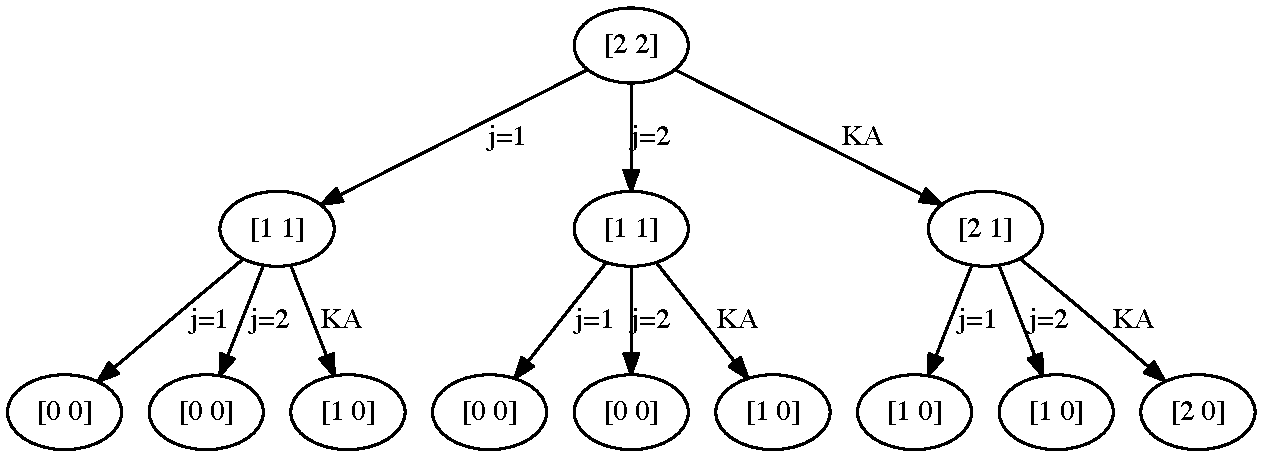
\includegraphics[width=140mm]{Bilder/Einfach.pdf}
    \caption{Rekursive Übergänge der Systemzustände ohne Memofunktion}  \label{Einfach}
        {\footnotesize \textbf{In Anlehnung an:} \cite{hetland2010python}, S. 179.} 
    {\footnotesize \textbf{Legende:} Annahme eines Produktauftrags entspricht '$j$', KA='Kein Auftrag'} 
  \end{center}
\end{figure}

Abbildung \ref{Einfach} zeigt die möglichen Systemzustände in Form der Knoten und die Übergänge in Form der Kanten. Dabei ist ein Knoten definiert als Zahlenfolge $[c_h\; t]$ und zeigt damit den Kapazitätsbestand $c_h$ zum Zeitpunkt $t$. Durch Annahme einer Produktanfrage $j\in\mathcal{J}$ oder sofern keine Anfrage eintrifft, wird ein Systemzustand verlassen. Diese rekursive Folge des Graphen wird konstruiert durch Anwenden der Gleichung \eqref{DP}. Sofern keine Memofunktion Anwendung findet, werden die einzelnen Teilprobleme jeweils mehrfach ermittelt, da sie jeweils für das vorherige Teilproblem notwendig sind.

\begin{figure}[h!]
  \begin{center}
    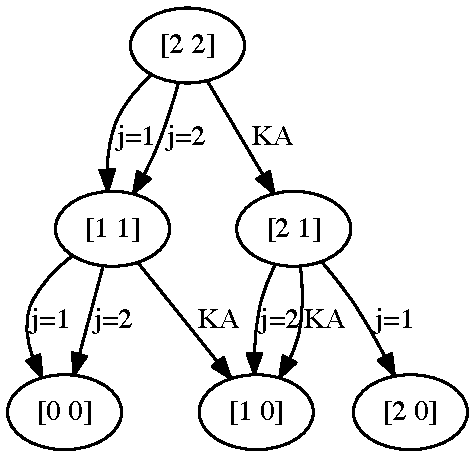
\includegraphics[width=50mm]{Bilder/Einfach2.pdf}
    \caption{Rekursive Übergänge mit Memofunktion}  \label{Einfach2}
        {\footnotesize \textbf{In Anlehnung an:} \cite{hetland2010python}, S. 179.} 
    {\footnotesize \textbf{Legende:} Annahme einer Produktauftrag entspricht '$j$', KA='Kein Auftrag'} 
  \end{center}
\end{figure}

Durch Anwenden einer Memofunktion können die möglichen Übergänge der Systemzustände des Beispiels reduziert werden, wie Abbildung \ref{Einfach2} zeigt. Jedes Systemzustand ist nur einmal im Zustandsraum vorhanden und sofern der rekursive Verlauf auf ein bereits ermitteltes Teilproblem trifft, erfolgt das Abrufen der bereits gespeicherten Lösung. Anders formuliert bedeutet dies, dass nachdem der Systemzustand bzw. das Teilproblem $[1\; 1]$ aufgrund der Anfrage nach Produkt $j=1$ gelöst ist, erfolgt keine Berechnung des gleichen Systemzustands $[1\; 1]$ aufgrund der Anfrage nach Produkt $j=2$. Das Ergebnis des Teilproblems wird direkt aus der Memofunktion abgerufen.

Der in dieser Arbeit verwendete \textbf{Algorithmus} zum exakten Lösen des Auftragsannahmeproblems im Netzwerk RM verwendet eine solche Memofunktion. Der Algorithmus berechnet den Erwartungswert des maximal möglichen Ertrags für ein Netzwerk RM auf Basis der rekursiven Form der Gleichung \eqref{time2}. Er durchläuft alle möglichen Teilprobleme bzw. Systemzustände des Netzwerks, indem der Algorithmus sich selbst mit angepassten Parametern aufruft. Als Grenzen für die rekursive Abfolge werden die Grenzbedingungen \eqref{GB1} und \eqref{GB2} hinterlegt. Das Lösen des Optimierungsproblems erfolgt damit durch Rückwärtsinduktion der rekursiven Folge, wobei bei jedem Teilproblem geprüft wird, ob bereits eine Lösung in der Memofunktion vorliegt. Nachfolgend wird der verwendete Algorithmus als Pseudocode dargestellt.


\begin{algorithm}[H]
%\renewcommand{\lstlistingname}{Code}
\textbf{Pseudocode: Auftragsannahmeproblem im Netzwerk RM;\\ 
Ermittlung des Erwartungswerts $V(\textbf{c}^{\hat t},\textbf{y}^{\hat t},t)$}\\
\Ein{$Memofunktion$}
\Ein{$\mathcal{H}$, $\mathcal{J}$, $T$, $\hat T$, $\textbf{c}^{\hat t}$, $\textbf{y}^{\hat t}$, $\textbf{a}^{\hat t}_j$, $r_{j}$, $p_j(t)$}
\uWenn{$V(\textnormal{\textbf c}^{\hat t},\textnormal{\textbf y}^{\hat t},t) \notin Memofunktion$}{
	\uWenn{$t \neq 0$}{
		$value^{reject} = V(\textbf{c}^{\hat t},\textbf{y}^{\hat t},t-1)$\\
		\FuerJedes{$j\in\mathcal{J}$}{
		% Accept
			\uWenn{$\textnormal{\textbf c}^{\hat t}-\textnormal{\textbf a}_j^{\hat t}\ge \textnormal{\textbf{0}}$}{
				$value_{j}^{accept} = p_j(t)\cdot\max[0,r_{j}-value^{reject}+V(\textnormal{\textbf c}^{\hat t}-\textnormal{\textbf a}^{\hat t}_j,\textbf{y}^{\hat t},t-1)]$}
			\uSonst{Grenzbedingung \eqref{GB2}: $V(\textnormal{\textbf c}^{\hat t}-\textnormal{\textbf a}^{\hat t}_j,\textbf{y}^{\hat t},t-1)=-\infty$\\
			$value_{j}^{accept} = p_j(t)\cdot\max[0,r_{j}-value^{reject}-\infty]$}
			% 2
			\uWenn{$\textnormal{\textbf y}^{\hat t}-Y(\textnormal{\textbf a}_j^{\hat t},\hat t)\ge \textnormal{\textbf{0}}$}{
				$value_{j}^{storage} = p_j(t)\cdot\max[0,r_{j}-value^{reject}+V(\textnormal{\textbf c}^{\hat t},\textbf{y}^{\hat t}-Y(\textnormal{\textbf a}^{\hat t}_j,\hat t),t-1)]$}
			\uSonst{Grenzbedingung \eqref{GB2}: $V(\textnormal{\textbf c}^{\hat t},\textbf{y}^{\hat t}-Y(\textnormal{\textbf a}^{\hat t}_j,\hat t),t-1)=-\infty$\\
			$value_{j}^{storage} = p_j(t)\cdot\max[0,r_{j}-value^{reject}-\infty]$}
				% 3
			\uWenn{$\textnormal{\textbf c}^{\hat t}-\textnormal{\textbf a}_j^{\hat t}\ge \textnormal{\textbf{0}} \textnormal{\textbf{ and }} \textnormal{\textbf y}^{\hat t}+Y(\textnormal{\textbf a}_j^{\hat t},\hat t +1)\le \textnormal{\textbf{y}}^{\hat t, max}$}{
				$value_{j}^{workup} = p_j(t)\cdot\max[0,V(\textnormal{\textbf c}^{\hat t}-\textnormal{\textbf a}^{\hat t}_j,\textbf{y}^{\hat t}+Y(\textnormal{\textbf a}_j^{\hat t},\hat t+1),t-1)-value^{reject}]$}
			\uSonst{Grenzbedingung \eqref{GB2}: $V(\textnormal{\textbf c}^{\hat t}-\textnormal{\textbf a}^{\hat t}_j,\textbf{y}^{\hat t}+Y(\textnormal{\textbf a}_j^{\hat t},\hat t+1),t-1)=-\infty$\\
			$value_{j}^{workup} = p_j(t)\cdot\max[0,-\infty-value^{reject}]$}
			
			}
			$list = [0]$\\
			\FuerJedes{$j\in\mathcal{J}$}{
			\uWenn{$p_j(t)>0$}{
			$list = list + [V(\textnormal{\textbf c}^{\hat t}-\textnormal{\textbf a}^{\hat t}_j,\textbf{y}^{\hat t}+Y(\textnormal{\textbf a}_j^{\hat t},\hat t+1),t-1)-value^{reject}]$
			}\uSonst{$list = list + [0]$}}
			
		$V(\textbf{c}^{\hat t},\textbf{y}^{\hat t},t)=value^{reject} + \sum_{j\in\mathcal{J}}(value_j^{accept}+value_j^{storage}+value_j^{workup})+p_0(t)\max [list]$}
	\uSonst{Grenzbedingung \eqref{GB1}: $V(\textbf{c}^{\hat t},\textbf{y}^{\hat t},t)=0$}
	$Memofunktion = Memofunktion+[V(\textbf{c}^{\hat t},\textbf{y}^{\hat t},t)]$}
\lSonst{$V(\textbf{c}^{\hat t},\textbf{y}^{\hat t},t) \textbf{ aus } Memofunktion$}
\Aus{$V(\textbf{c}^{\hat t},\textbf{y}^{\hat t},t)$}
%{\footnotesize \textbf{Quelle:} \cite{bouleimen2003new}, S. 273}
\end{algorithm}

Bei der Implementierung des Algorithmus zum Lösen der Modellerweiterung des Auftragsannahmeproblems im Netzwerk RM mit Lagerhaltungsentscheidungen wurde die Programmiersprache \texttt{Python/2.7.1} verwendet. Es handelt sich um eine höhere Programmiersprache mit einem Interpreter.\footnote{Vgl. \cite{:2005aa}, S. 8.} Als  Kommandozeileninterpreter wird in dieser Arbeit \texttt{IPython/3.2.1} genutzt. Zur Verbesserung der Laufzeit der Implementierung wird auf die Programmbibliothek \texttt{NumPy/}\texttt{1.9.2} zurückgegriffen. Mit dieser Programmbibliothek ist es möglich multidimensionale Datenstrukturen zu formen und mit den integrierten numerischen Algorithmen sowie mathematischen Werkzeugen zu bearbeiten.\footnote{Vgl. \cite{lindblad2013numpy}, S. 35-49.} Zusätzlich wird die \texttt{Python}-Bibliothek \texttt{SciPy/0.15.1} genutzt, die weitere Werkzeuge für die \texttt{NumPy}-Datenstrukturen liefert.\footnote{Vgl. \cite{lindblad2013numpy}, S. 49-52.} Die Laufzeitverbesserung kommt zu Stande, da die Funktionen der Programmbibliothek auf homogene Datenstrukturen zurückgreifen.\footnote{Vgl. \cite{:2006aa}, S. 131.} Damit lassen sich annähernd ähnliche Ergebnisse wie mit \texttt{Fortran}, \texttt{C} und \texttt{C++} erzielen, wobei weiterhin die einfache Syntax von \texttt{Python/2.7.1} besteht. Zusätzlich wird die Programmbibliothek \texttt{NetworkX/1.9.1} verwendet, um die ermittelten Erwartungswerte in eine Netzwerkdatenstruktur zu überführen. Diese Netzwerkdatenstruktur ist explizit für Multigraphen geeignet, was für diese Problemstellung notwendig ist. Die Teilprobleme werden miteinander in Beziehung gesetzt, indem ein Teilproblem ein Knoten bildet und die für das Teilproblem notwendigen nachfolgenden Teilprobleme die Kanten der Netzwerkdatenstruktur bilden. Dadurch wird das Optimierungsproblem als Netzwerk interpretierbar. Weiter kann dieser Netzwerkdatenstruktur grafisch expotiert werden, indem eine für das Programm \texttt{GraphViz/2.38.0} verwertbare Datei erzeugt wird. Dadurch ist das Rendern der jeweiligen Netzwerkdatenstruktur möglich. Sämtliche in dieser Arbeit abgebildeten Graphen sind mit dem Programm \texttt{GraphViz/2.38.0} erstellt. Zusätzlich erfolgt die Verwaltung der Daten durch die Datenanalyse-Programmbibliothek \texttt{Pandas/0.16.2}.

%Das Optimierungsmodell verwendet eine parallele Programmierung, womit die Laufzeit jedoch nur im geringen Maße verbessert wird. Dieser Sachverhalt und die numerische Untersuchung des Algorithmus für die Auftragsannahme von auftragsbezogenen Instandhaltungsprozessen anhand von Szenarien sind im Abschnitt \ref{Untersuchung} aufgeführt. Im Vorfeld muss jedoch die Erweiterung des Grundmodells um das Entscheidungsproblem der Instandhaltung von Produkten erfolgen. Dies wird im nachfolgenden Abschnitt \ref{Umformung} durchgeführt.




